\setcounter{figure}{0}
\setcounter{table}{0}
\renewcommand{\thefigure}{S\arabic{figure}}
\renewcommand{\thetable}{S\arabic{table}}

\section*{Supplemental Material}

\subsection*{Supplemental Figures}

\begin{figure}[H]
  \begin{center}
  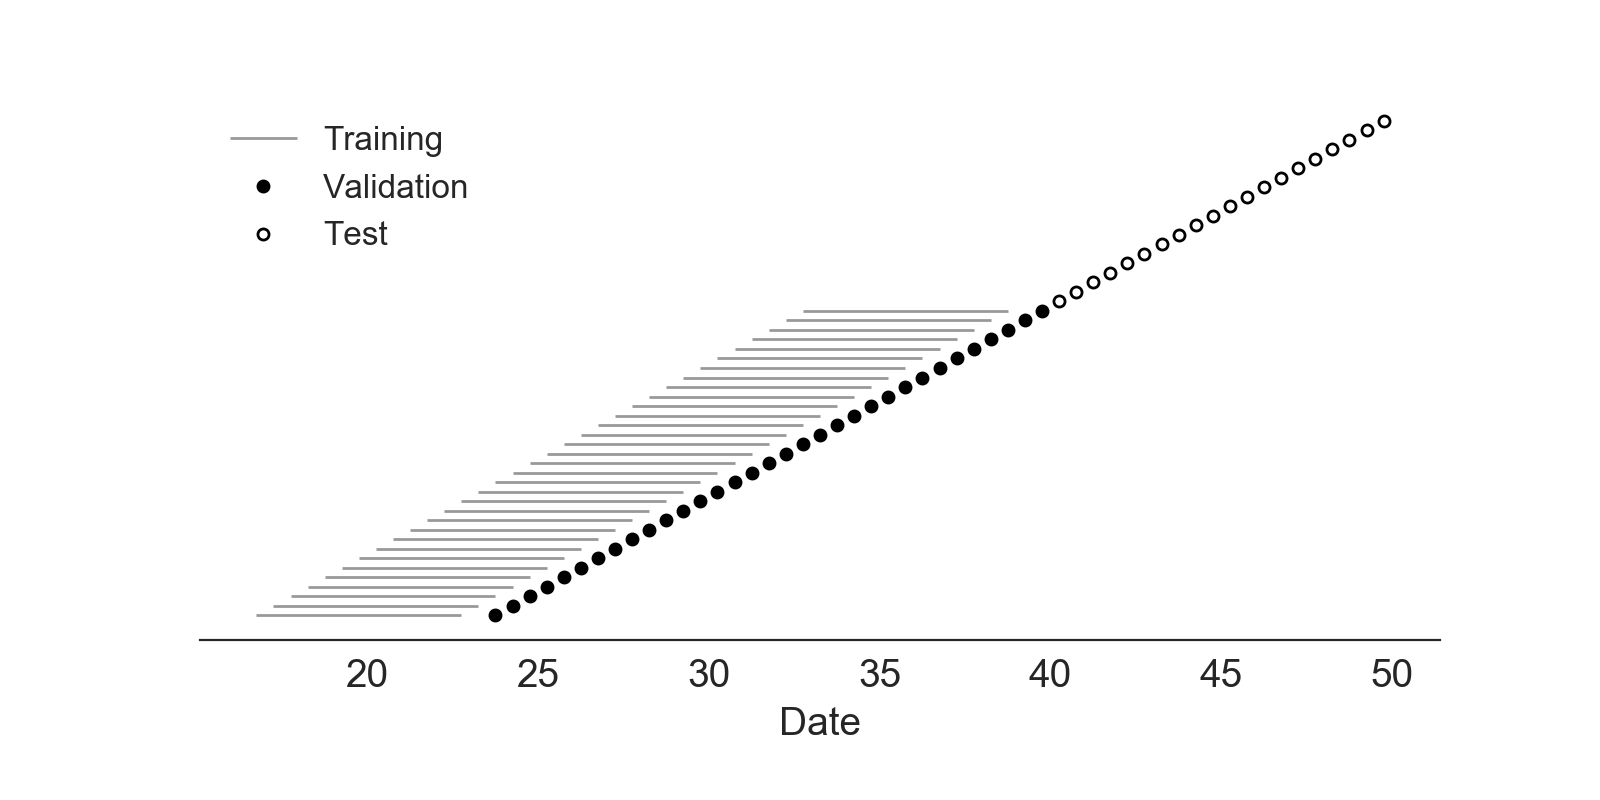
\includegraphics[width=\textwidth]{figures/cross-validation-for-simulated-populations.png}
  \caption{
  Time-series cross-validation scheme for simulated populations.
  Models were trained in six-year sliding windows (grey lines) and validated on out-of-sample data from validation timepoints (filled circles).
  Validation results from 30 years of data were used to iteratively tune model hyperparameters.
  After fixing hyperparameters, model coefficients were fixed at the mean values across all training windows.
  Fixed coefficients were applied to 10 years of new out-of-sample test data (open circles) to estimate true forecast errors.
  }
  \label{sup_fig:cross_validation_for_simulated_populations}
  \end{center}
\end{figure}

\begin{figure}[H]
  \begin{center}
  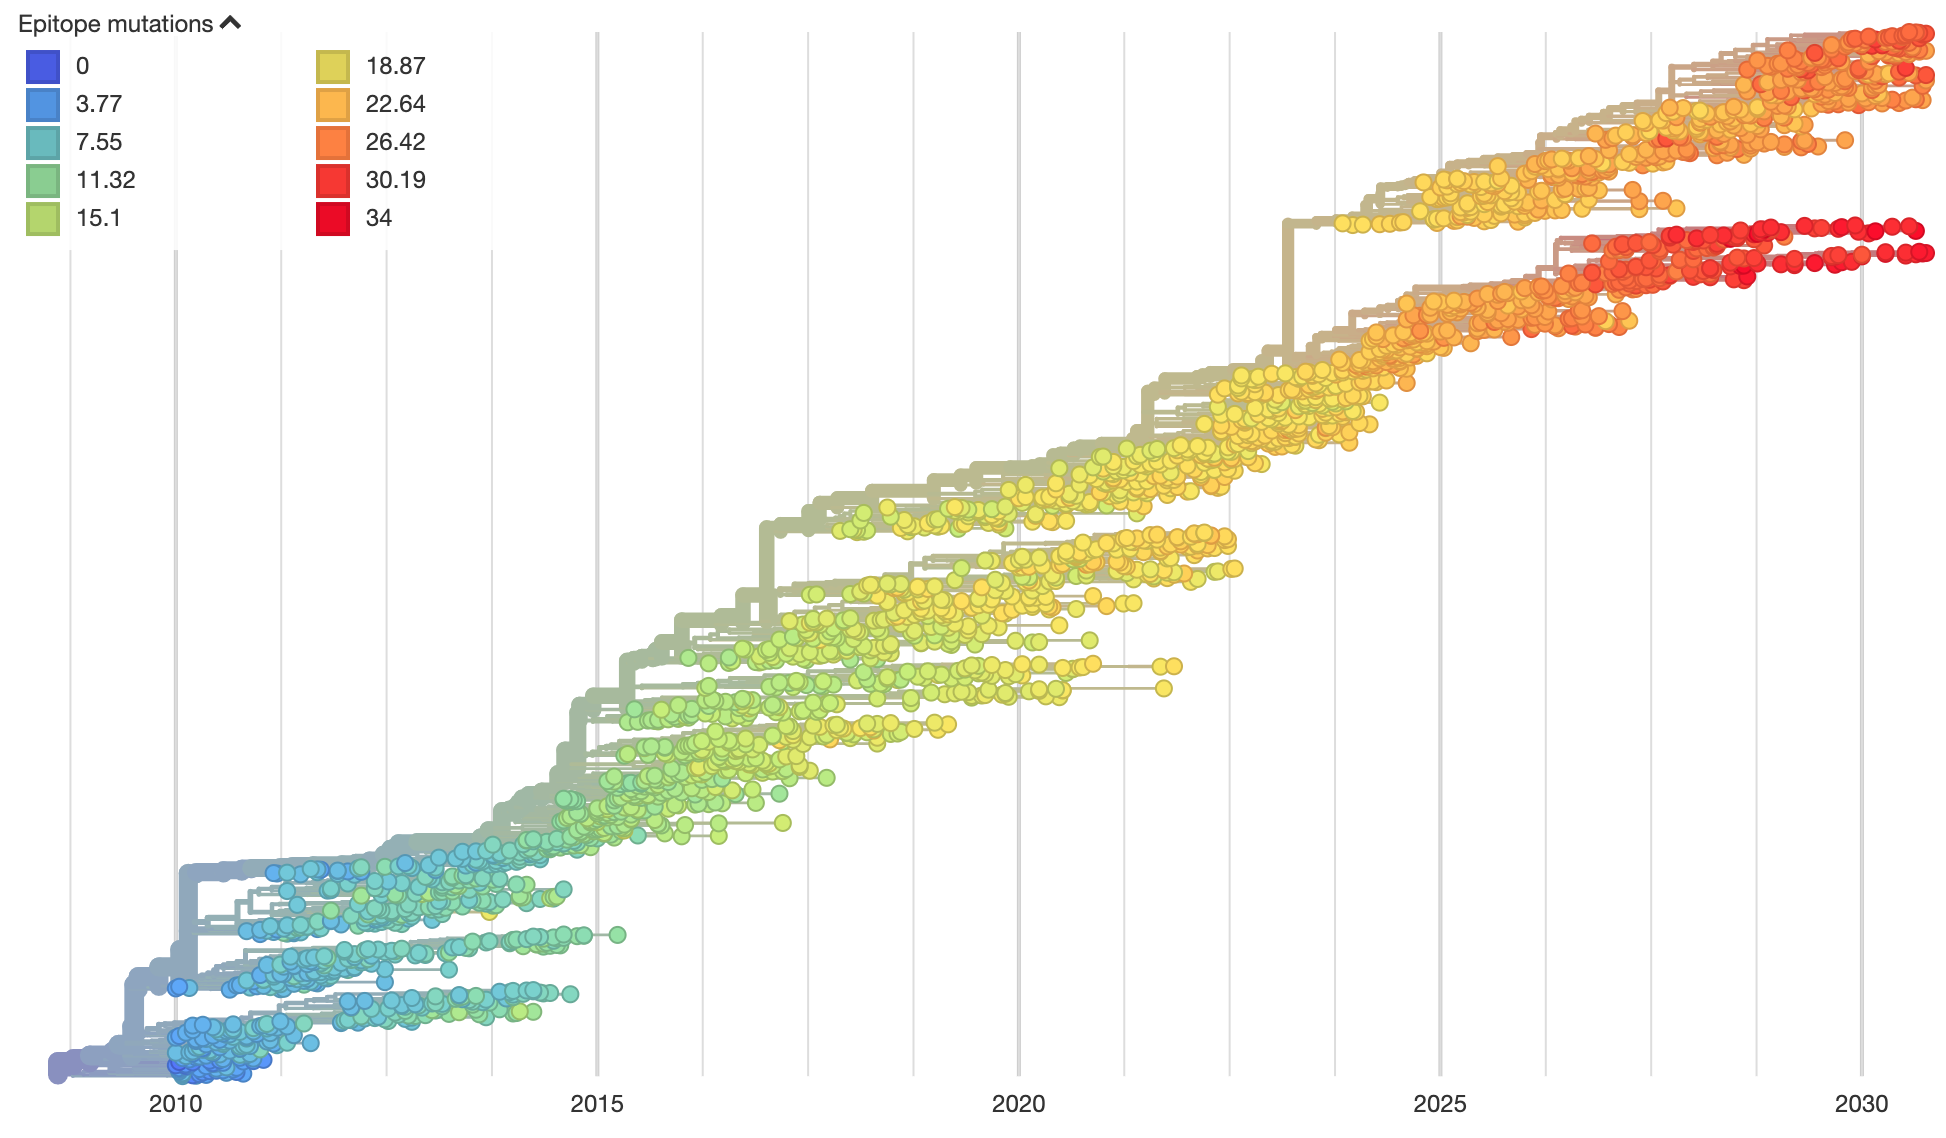
\includegraphics[width=\textwidth]{figures/simulated-h3n2-ha-phylogeny.png}
  \caption{
  Phylogeny of H3N2-like HA sequences sampled between the 24th and 30th years of simulated evolution.
  The phylogenetic structure and rate of accumulated epitope and non-epitope mutations match patterns observed in phylogenies of natural sequences.
  Sample dates were annotated as the generation in the simulation divided by 200 and added to 2000, to acquire realistic date ranges that were compatible with our modeling machinery.
  }
  \label{sup_fig:simulated_h3n2_ha_phylogeny}
  \end{center}
\end{figure}

\begin{figure}[H]
  \begin{center}
  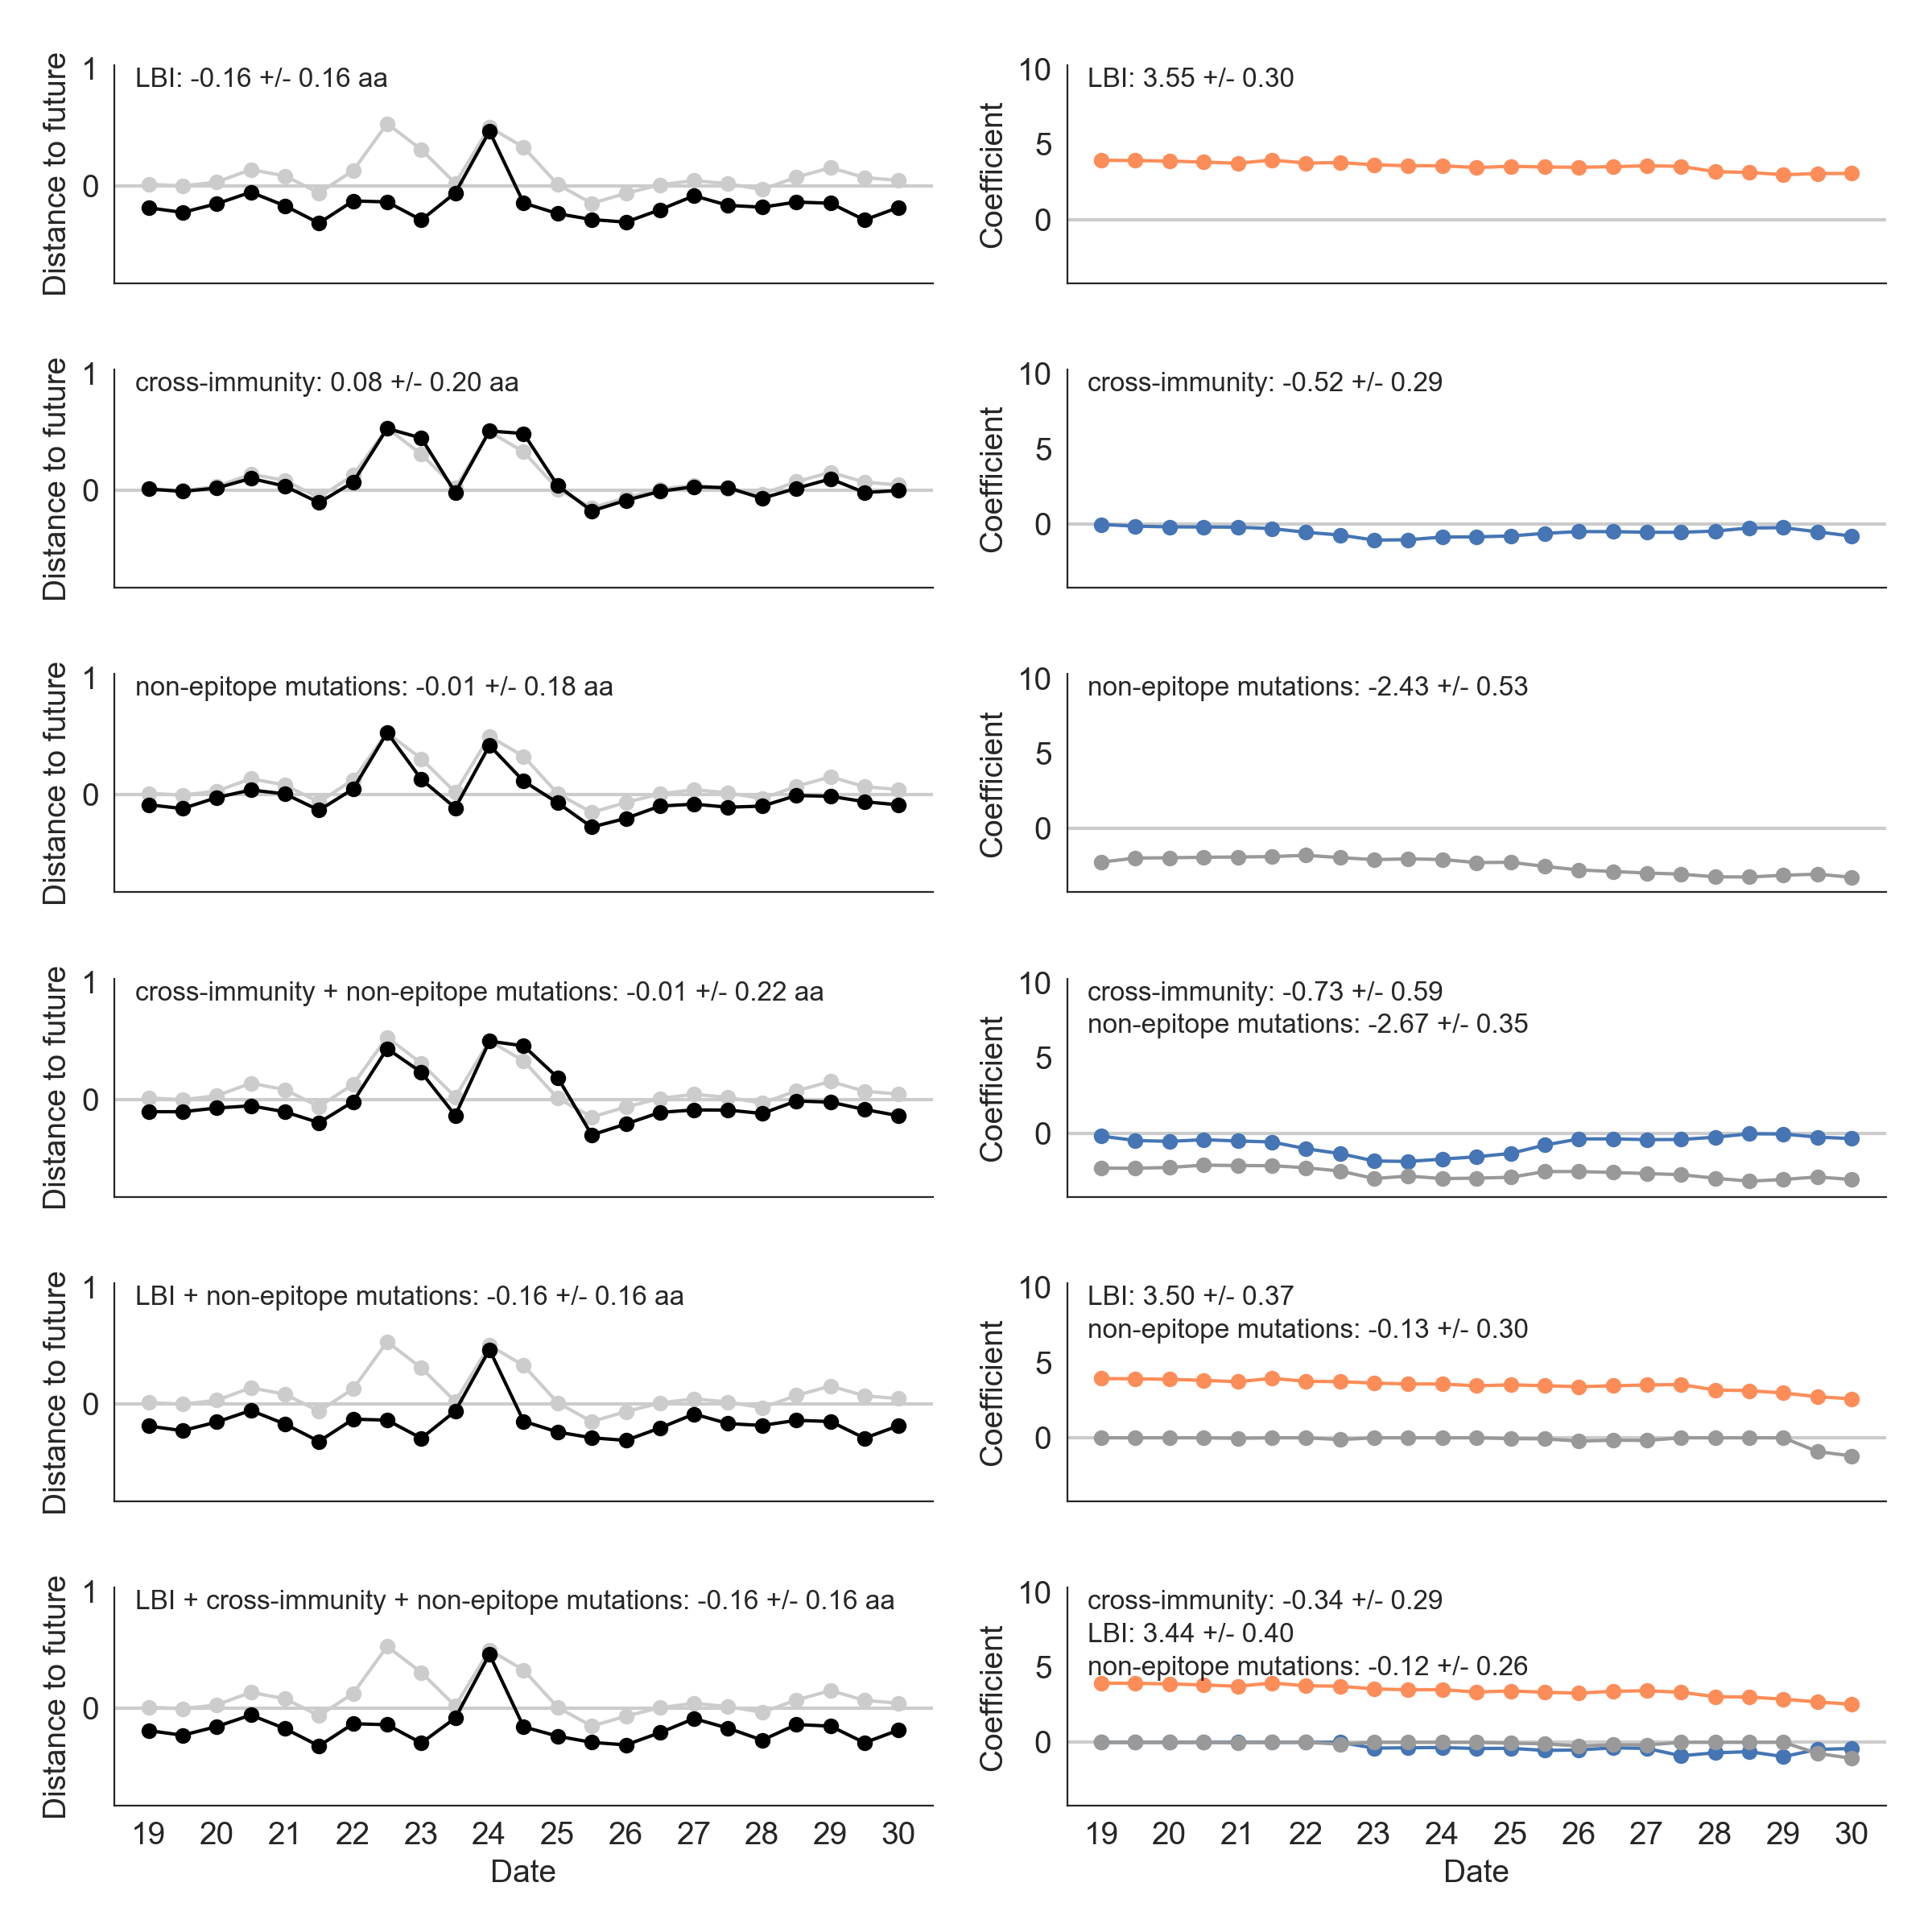
\includegraphics[width=\textwidth]{figures/unadjusted-composite-model-accuracy-and-coefficients-for-simulated-populations.png}
  \caption{
  Composite model coefficients and distances to the future for models fit to simulated populations.
  A) Coefficients and B) distances are shown per validation timepoint and test timepoint as in Fig.~\ref{fig:unadjusted_model_accuracy_and_coefficients_for_simulated_populations_controls}.
  }
  \label{sup_fig:unadjusted_composite_model_accuracy_and_coefficients_for_simulated_populations}
  \end{center}
\end{figure}

\begin{figure}[H]
  \begin{center}
  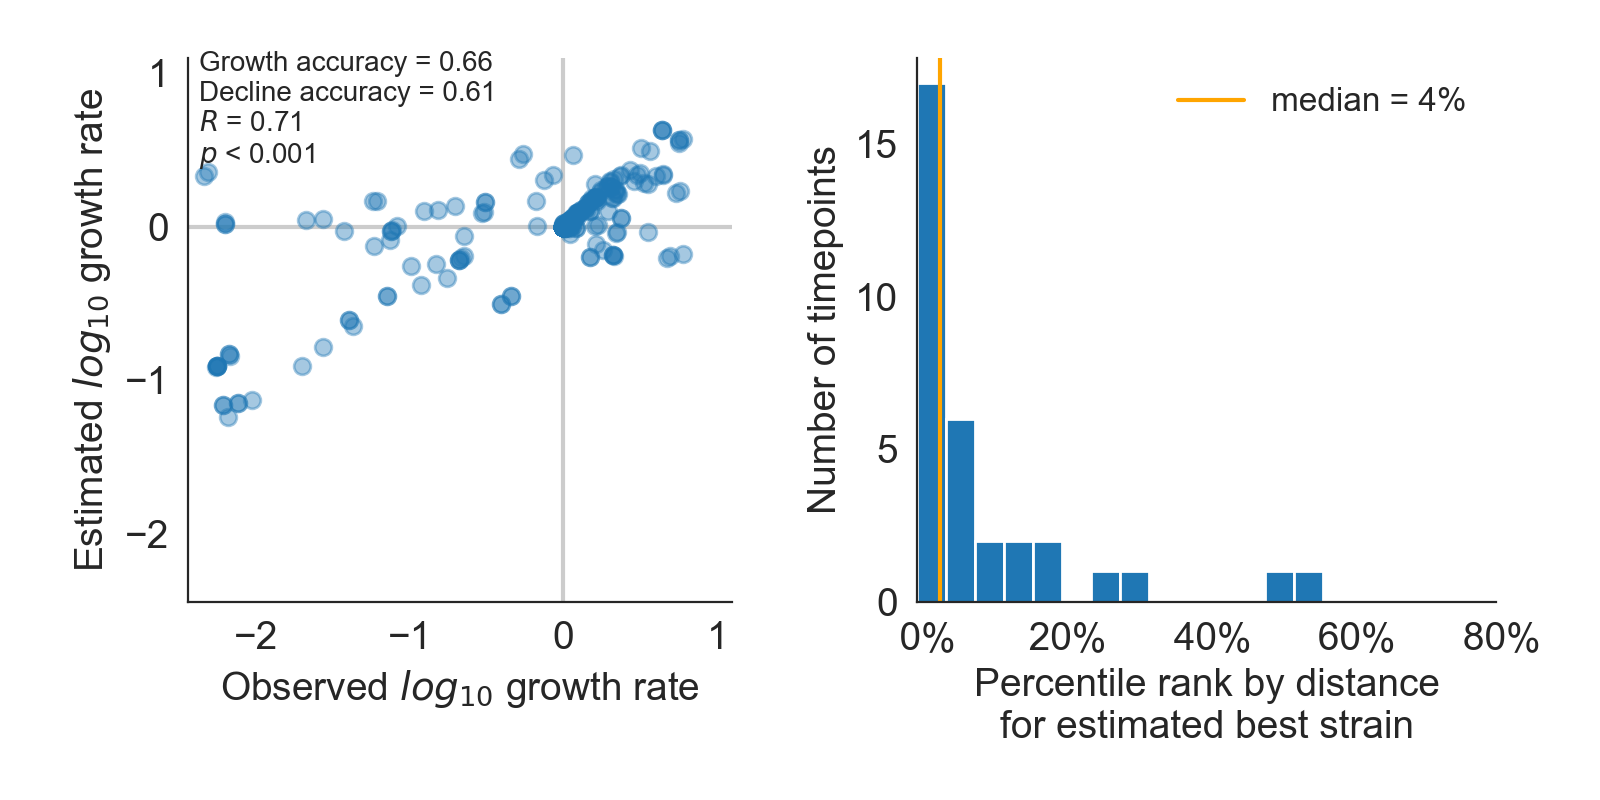
\includegraphics[width=\textwidth]{figures/validation-of-best-model-for-simulated-populations.png}
  \caption{
  Validation of best model for simulated populations of H3N2-like viruses.
  A) The correlation of estimated and observed clade growth rates shows the model's ability to capture clade-level dynamics without explicitly optimizing for clade frequency targets.
  B) The rank of the estimated best strain based on its distance to the future for 33 timepoints.
  The estimated best strain was in the top 20th percentile of observed closest strains for 100\% of timepoints, confirming that the model makes a good choice when forced to select a single representative strain for the future population.
  C) Absolute forecast error for clades shown in A by their initial frequency with a mean LOESS fit (solid black line) and 95\% confidence intervals (grey shading) based on 100 bootstraps.
  D) The correlation of all strains at all timepoints by the percentile rank of their observed and estimated distances to the future.
  }
  \label{sup_fig:validation_of_best_model_for_simulated_populations}
  \end{center}
\end{figure}

\begin{figure}[H]
  \begin{center}
  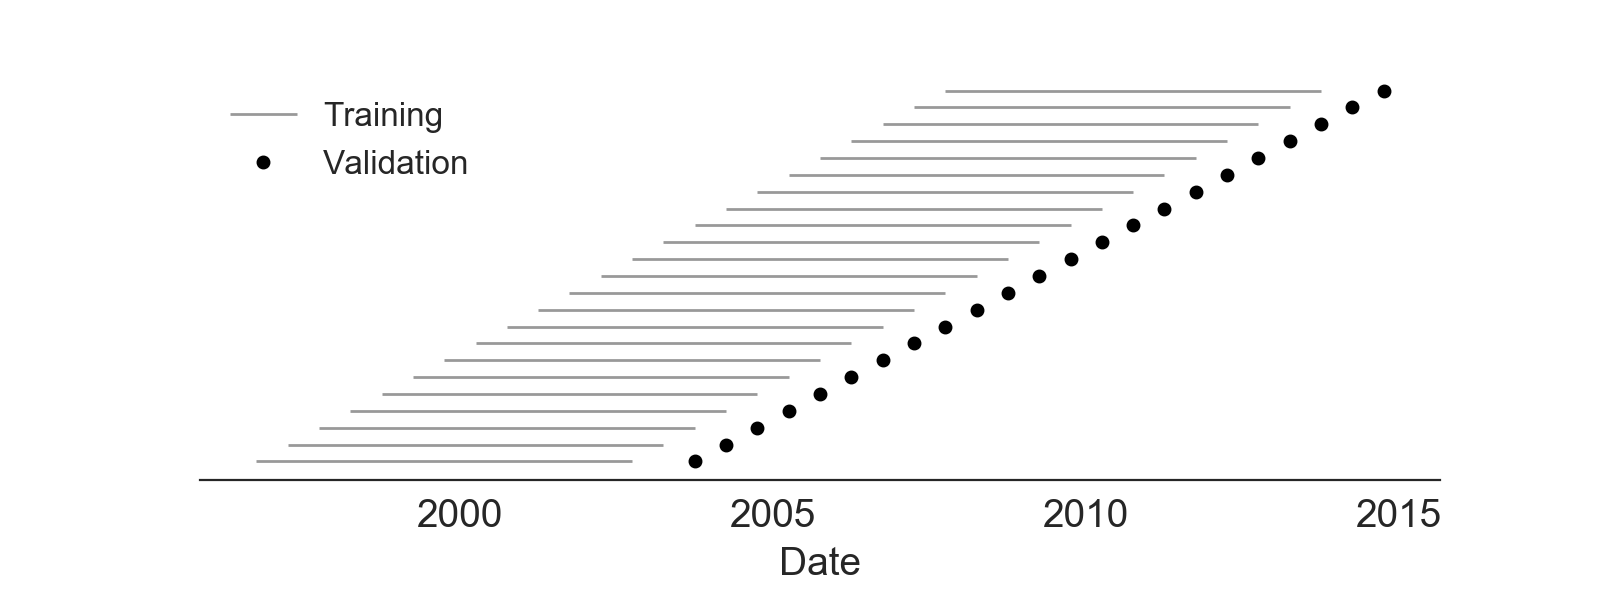
\includegraphics[width=\textwidth]{figures/cross-validation-for-natural-populations.png}
  \caption{
  Time-series cross-validation scheme for natural populations.
  Models were trained in six-year sliding windows (grey lines) and validated on out-of-sample data from validation timepoints (filled circles).
  Validation results from 25 years of data were used to iteratively tune model hyperparameters.
  After fixing hyperparameters, model coefficients were fixed at the mean values across all training windows.
  Fixed coefficients were applied to four years of new out-of-sample test data (open circles) to estimate true forecast errors.
  }
  \label{sup_fig:cross_validation_for_natural_populations}
  \end{center}
\end{figure}

\begin{figure}[H]
  \begin{center}
  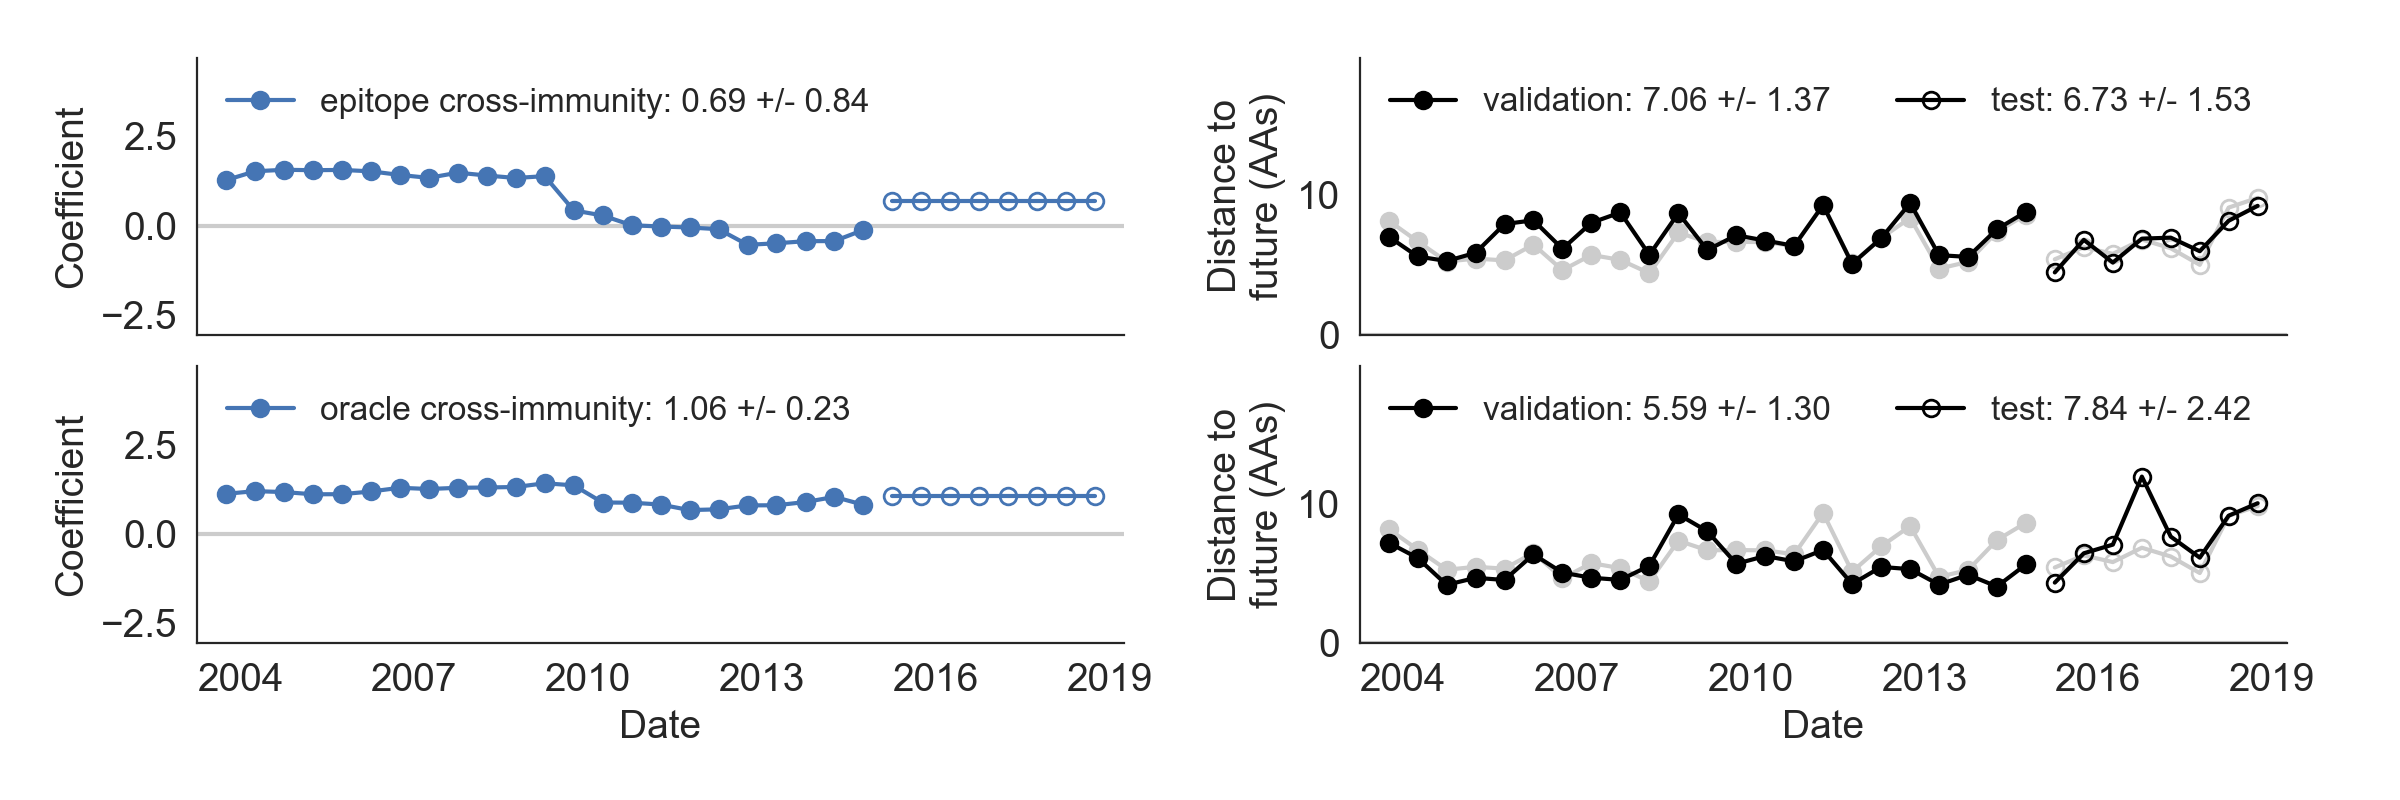
\includegraphics[width=\textwidth]{figures/unadjusted-composite-model-accuracy-and-coefficients-for-natural-populations-epitope-vs-oracle.png}
  \caption{
  Model coefficients and distances to the future for cross-immunity models fit to natural populations.
  A) Coefficients and B) distances are shown per validation timepoint and test timepoint as in Fig.~\ref{fig:unadjusted_model_accuracy_and_coefficients_for_simulated_populations_controls}.
  The epitope cross-immunity model relies on previously published epitope sites \cite{Luksza:2014hj}.
  The ``oracle'' cross-immunity model relies on sites of beneficial mutations that were manually identified from the entire training and validation time period (Methods).
  The improved performance of the ``oracle'' model indicates that the sequence-based cross-immunity metric can be effective when sites of beneficial mutations are known prior to forecasting.
  }
  \label{sup_fig:unadjusted_composite_model_accuracy_and_coefficients_for_natural_populations_epitope_vs_oracle}
  \end{center}
\end{figure}

\begin{figure}[H]
  \begin{center}
  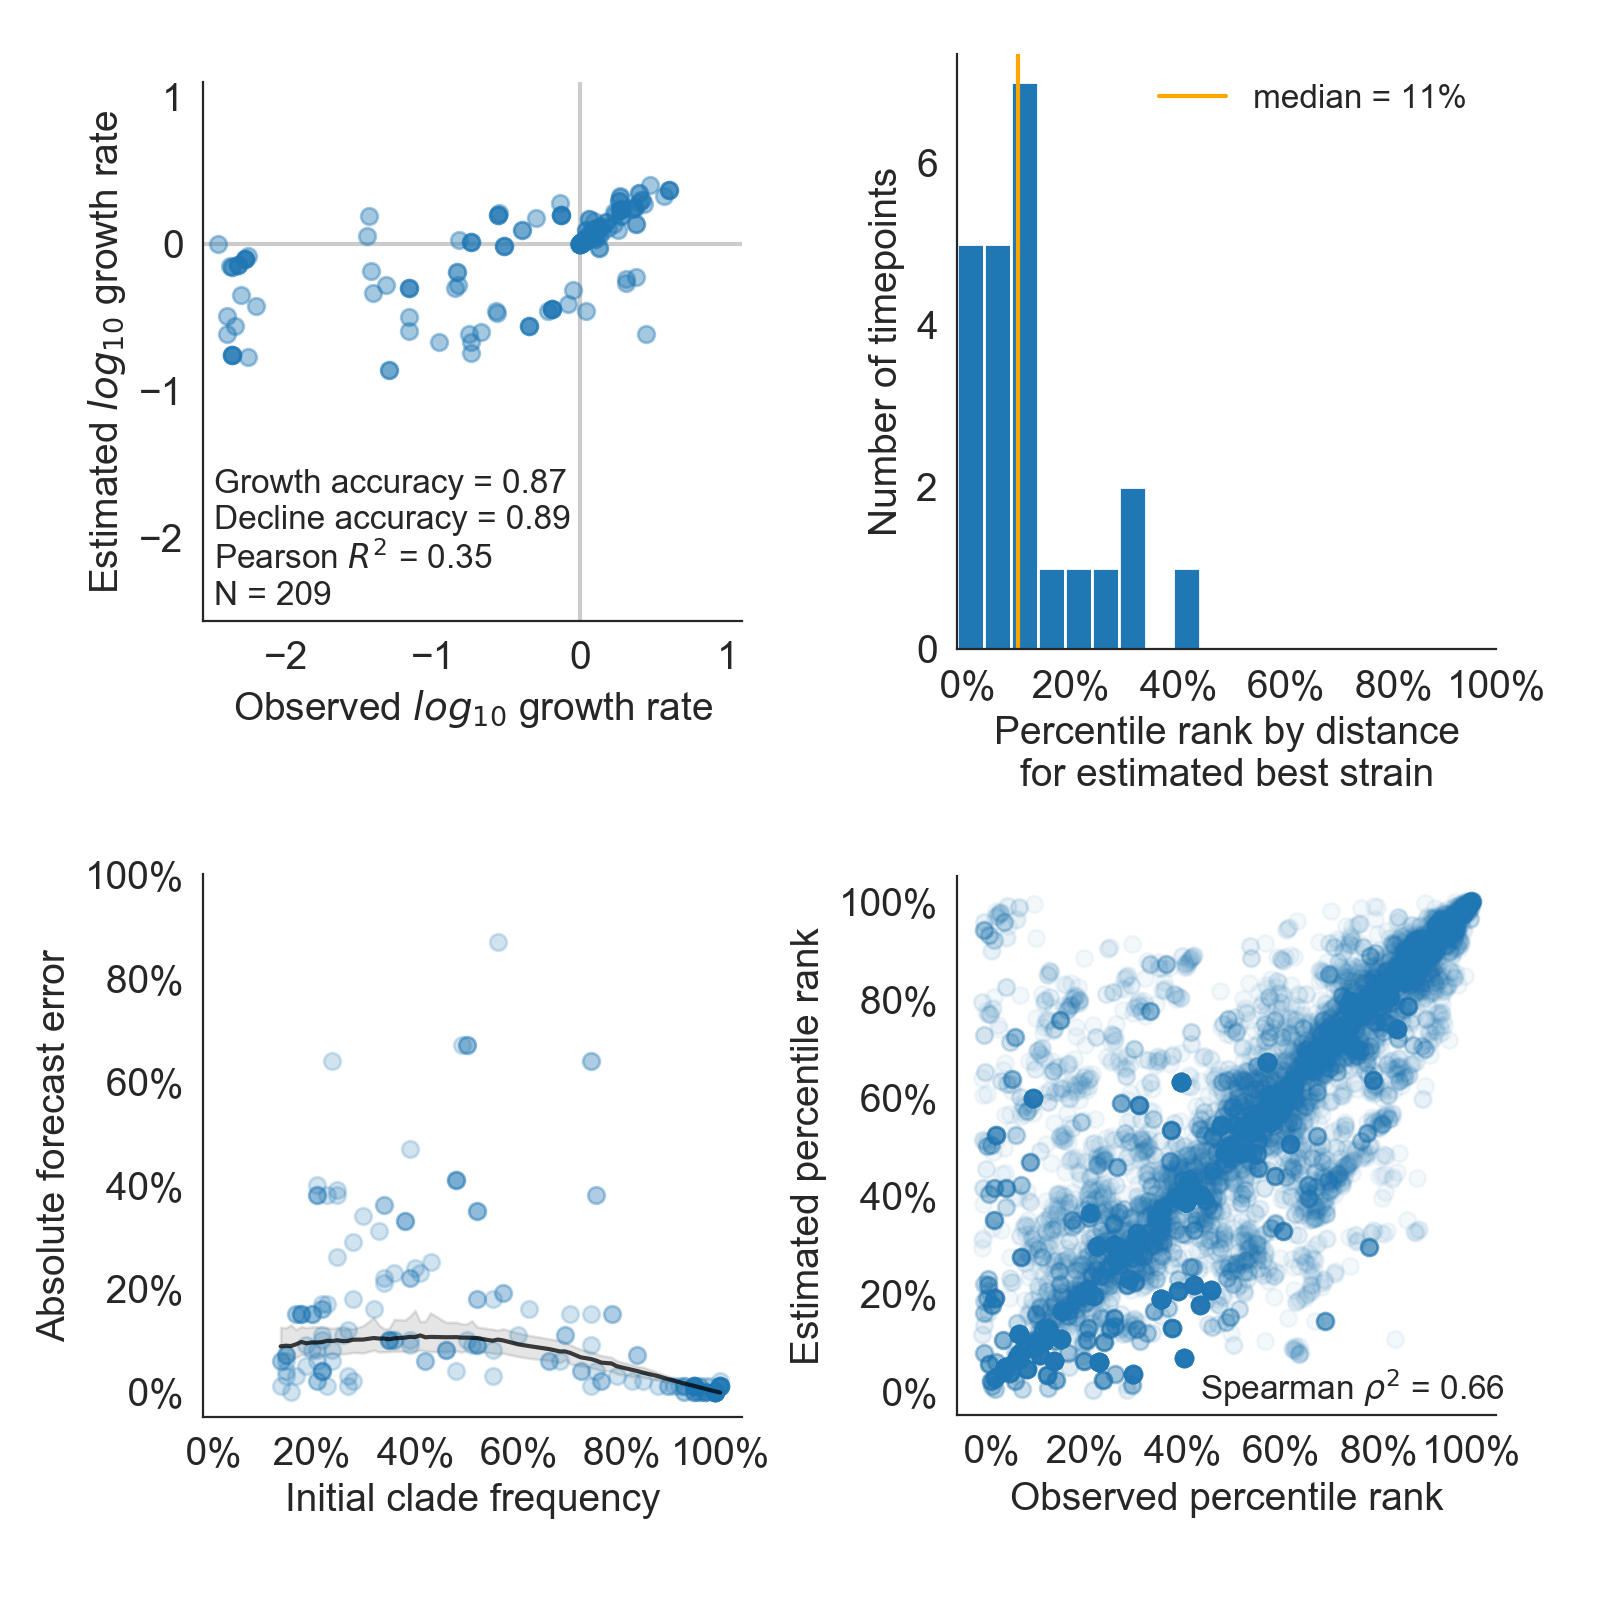
\includegraphics[width=\textwidth]{figures/validation-of-best-model-for-natural-populations.png}
  \caption{
  Validation of best model for natural populations of H3N2 viruses, the composite model of mutational load and LBI.
  A) The correlation of estimated and observed clade growth rates shows the model's ability to capture clade-level dynamics without explicitly optimizing for clade frequency targets.
  B) The rank of the estimated best strain based on its distance to the future for 23 timepoints.
  The estimated best strain was in the top 20th percentile of observed closest strains for 87\% of timepoints, confirming that the model makes a good choice when forced to select a single representative strain for the future population.
  C) Absolute forecast error for clades shown in A by their initial frequency with a mean LOESS fit (solid black line) and 95\% confidence intervals (grey shading) based on 100 bootstraps.
  D) The correlation of all strains at all timepoints by the percentile rank of their observed and estimated distances to the future.
  }
  \label{sup_fig:validation_of_best_model_for_natural_populations}
  \end{center}
\end{figure}

\begin{figure}[H]
  \begin{center}
  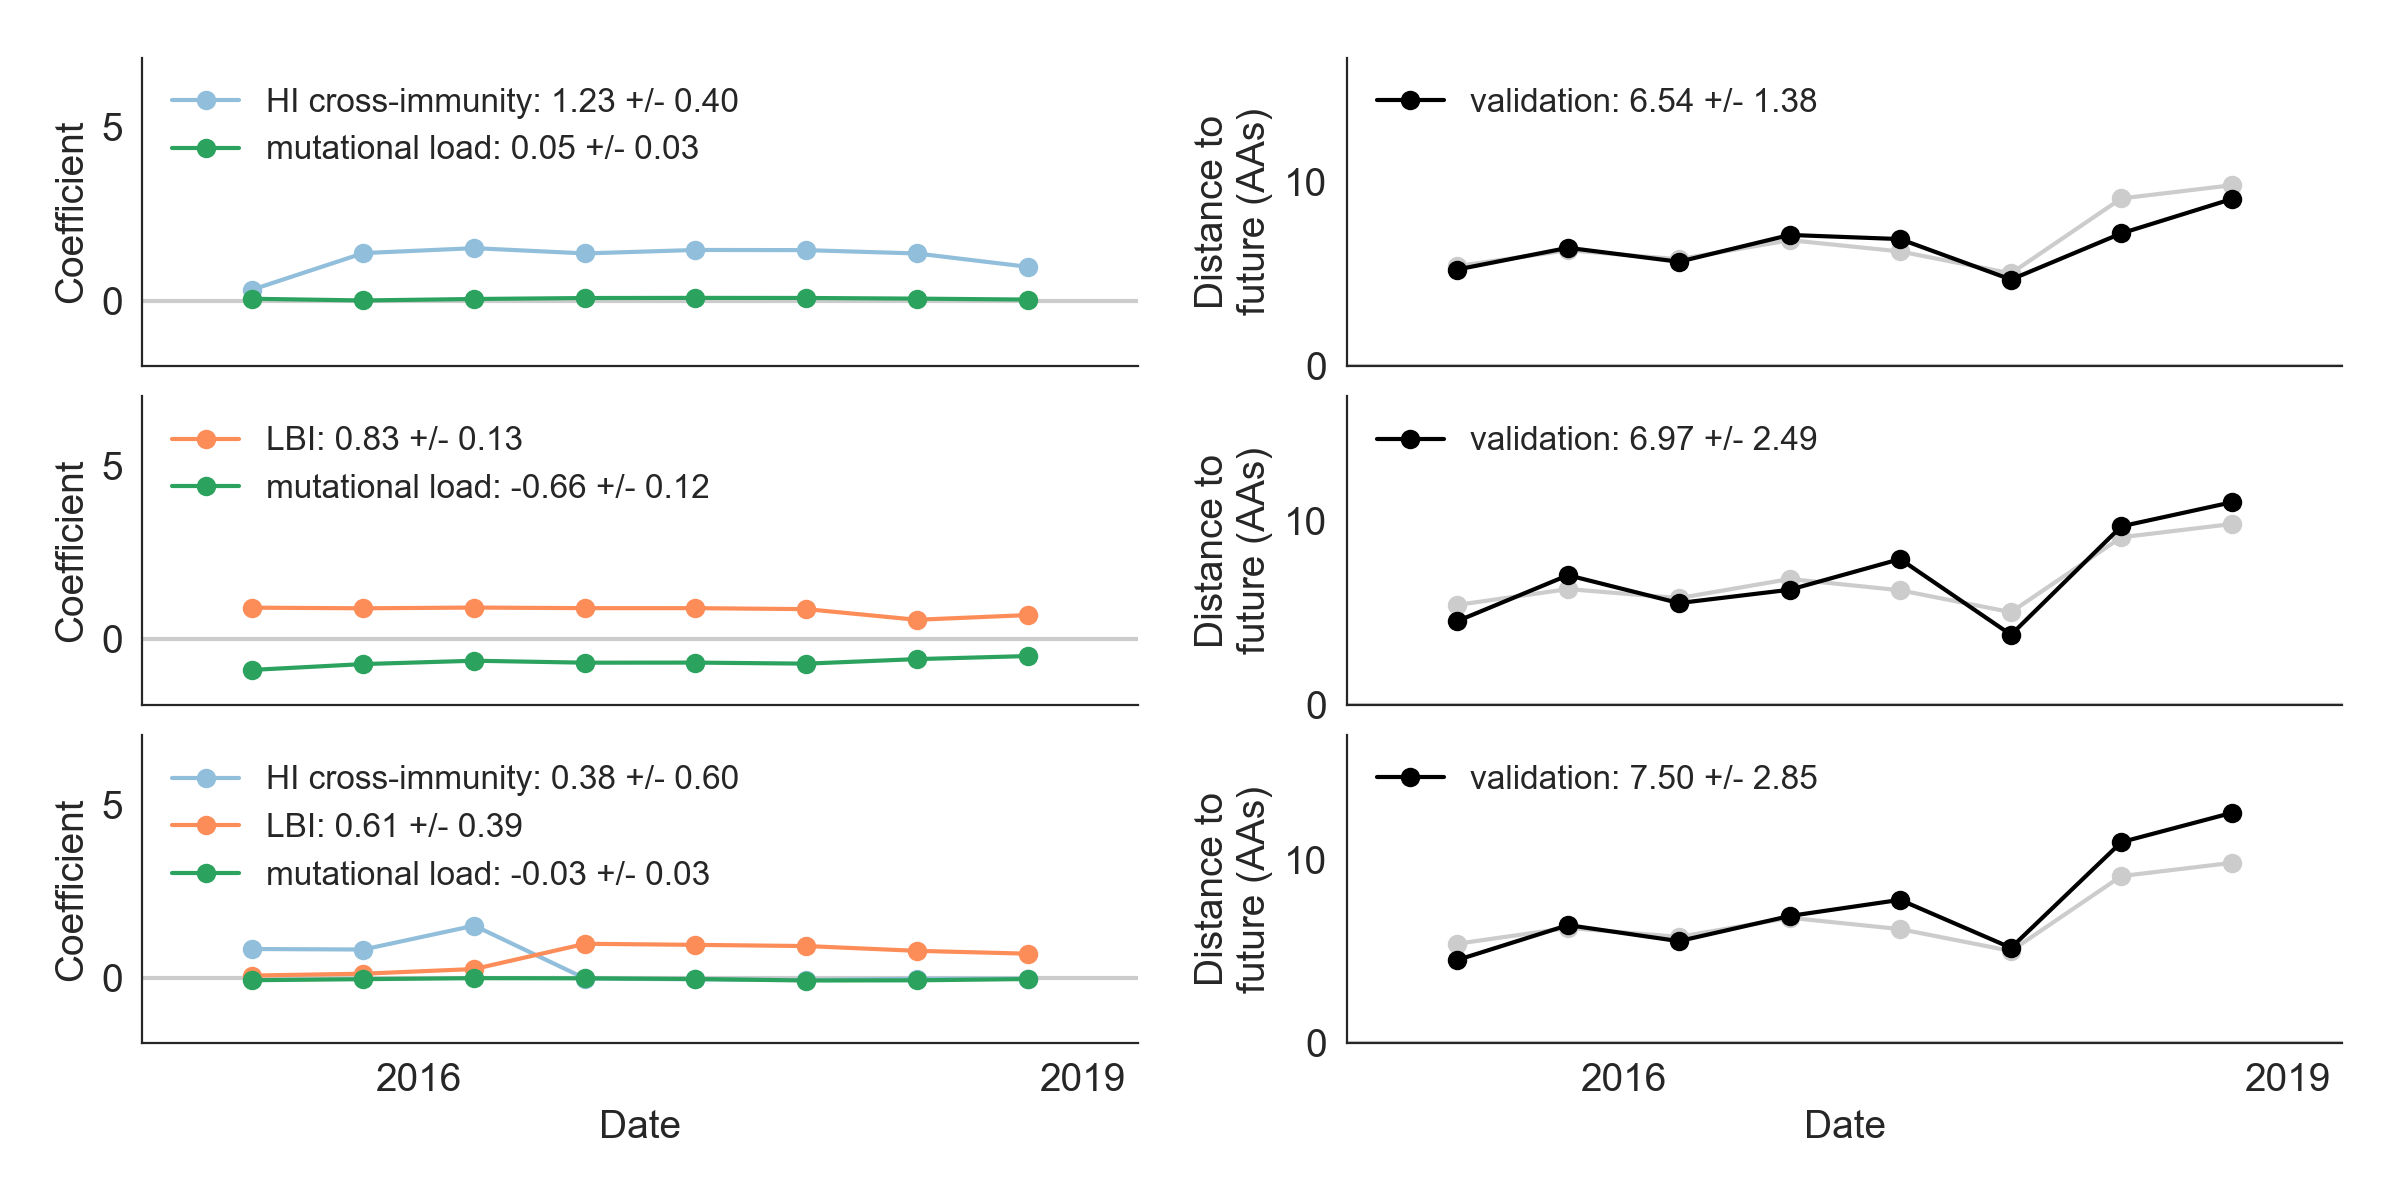
\includegraphics[width=\textwidth]{figures/models-natural-populations-composite-with-updated-coefficients-across-test-data.png}
  \caption{
    Model coefficients and distances to the future for best composite models and a FRA-based composite fit to recent data from natural populations as in Fig.~\ref{fig:unadjusted_model_accuracy_and_coefficients_for_simulated_populations_controls}.
    A) Coefficients and B) distances are shown per test timepoint (N=8).
    In contrast to the results for these models based on fixed coefficients from training/validation, these coefficients were learned for each six-year window prior to the corresponding test timepoint.
    The corresponding distances reflect the model's performance with updated coefficients on what is effectively new validation data.
    The naive model's distance to the future was 6.82 $\pm$ 1.74 AAs for these timepoints.
  }
  \label{sup_fig:updated_model_accuracy_and_coefficients_for_natural_populations_across_test_data}
  \end{center}
\end{figure}

\subsection*{Supplemental Tables}

\begin{table}[H]
  \begin{center}
    \begin{tabular}{lrrr}
\toprule
{} &  epitope mutations &  non-epitope mutations &  epitope-to-non-epitope ratio \\
branch type &                    &                        &                               \\
\midrule
side branch &                590 &                   1327 &                          0.44 \\
trunk       &                 23 &                     12 &                          1.92 \\
\bottomrule
\end{tabular}

    \caption{
    Number of epitope and non-epitope mutations per branch by trunk or side branch status for simulated populations.
    Epitope sites were defined previously described \cite{Luksza:2014hj}.
    Annotation of trunk and side branch was performed as previously described \cite{Bedford:2015fj}.
    Mutations were calculated for the full validation tree for simulated sequences samples between October of years 10 and 40.
    }
    \label{sup_table:mutations_by_trunk_status_for_simulated_populations}
  \end{center}
\end{table}

\begin{table}[H]
  \begin{center}
    \begin{tabular}{lrrr}
\toprule
{} &  epitope mutations &  non-epitope mutations &  epitope-to-non-epitope ratio \\
branch type &                    &                        &                               \\
\midrule
side branch &                485 &                   1177 &                          0.41 \\
trunk       &                 50 &                     32 &                          1.56 \\
\bottomrule
\end{tabular}

    \caption{
    Number of epitope and non-epitope mutations per branch by trunk or side branch status for natural populations.
    Epitope sites were defined previously described \cite{Luksza:2014hj}.
    Annotation of trunk and side branch was performed as previously described \cite{Bedford:2015fj}.
    Mutations were calculated for the full validation tree for natural sequences samples between 1990 and 2015.
    }
    \label{sup_table:mutations_by_trunk_status}
  \end{center}
\end{table}

\begin{table}[H]
  \begin{center}
    \scalebox{0.9}{
        \begin{tabular}{lll}
\toprule
                                           Model & \makecell{Distance closer \\ to future (AAs)} & \makecell{Model $>$ naive \\ (N=23)} \\
\midrule
                     non-epitope mutations + LBI &                                 0.96 +/- 1.42 &                            18 (78\%) \\
                                             LBI &                                 0.72 +/- 1.51 &                            17 (74\%) \\
       HI cross-immunity + non-epitope mutations &                                 0.63 +/- 0.79 &                            18 (78\%) \\
 HI cross-immunity + non-epitope mutations + LBI &                                 0.52 +/- 0.83 &                            19 (83\%) \\
                                         HI tree &                                 0.40 +/- 0.82 &                            15 (65\%) \\
                               HI cross-immunity &                                 0.36 +/- 0.65 &                            17 (74\%) \\
                                 delta frequency &                                 0.27 +/- 0.67 &                            16 (70\%) \\
                           non-epitope mutations &                                 0.26 +/- 0.56 &                            17 (74\%) \\
                          Koel epitope mutations &                                 0.19 +/- 0.25 &                            19 (83\%) \\
                                     DMS entropy &                                 0.02 +/- 0.15 &                            14 (61\%) \\
                                 DMS non-epitope &                                -0.05 +/- 0.15 &                             7 (30\%) \\
                        linear HI mut phenotypes &                                -0.06 +/- 0.51 &                            11 (48\%) \\
                           HI sub cross-immunity &                                -0.14 +/- 0.57 &                            10 (43\%) \\
                          Wolf epitope mutations &                                -0.17 +/- 0.31 &                             5 (22\%) \\
                          DMS mutational effects &                                -0.35 +/- 1.65 &                            11 (48\%) \\
                               epitope mutations &                                -0.43 +/- 0.94 &                             5 (22\%) \\
  epitope cross-immunity + non-epitope mutations &                                -0.54 +/- 1.39 &                             6 (26\%) \\
                          epitope cross-immunity &                                -0.66 +/- 1.13 &                             6 (26\%) \\
\bottomrule
\end{tabular}

    }
    \caption{
      All model coefficients and performance on validation and test data for natural populations ordered from best to worst by distance to the future, as in Table~\ref{table_simulated_model_selection}.
      Validation results are based on 23 timepoints.
      Test results are based on 8 timepoints not observed during model training and validation.
      Model results for additional variants of fitness metrics including those based on epitope mutations and DMS preferences are included for reference.
    }
    \label{sup_table:complete_natural_model_selection}
  \end{center}
\end{table}

\pagebreak

\subsection*{Supplemental Text}

\subsubsection*{GISAID Acknowledgements}

WHO Collaborating Centre for Reference and Research on Influenza, Victorian Infectious Diseases Reference Laboratory, Australia; WHO Collaborating Centre for Reference and Research on Influenza, Chinese National Influenza Center, China; WHO Collaborating Centre for Reference and Research on Influenza, National Institute of Infectious Diseases, Japan; The Crick Worldwide Influenza Centre, The Francis Crick Institute, United Kingdom; WHO Collaborating Centre for the Surveillance, Epidemiology and Control of Influenza, Centers for Disease Control and Prevention, United States; ADImmune Corporation, Taiwan; ADPH Bureau of Clinical Laboratories, United States; Aichi Prefectural Institute of Public Health, Japan; Akershus University Hospital, Norway; Akita Research Center for Public Health and Environment, Japan; Alabama State Laboratory, United States; Alaska State Public Health Laboratory, United States; Alaska State Virology Lab, United States; Aomori Prefectural Institute of Public Health and Environment, Japan; Aristotelian University of Thessaloniki, Greece; Arizona Department of Health Services, United States; Arkansas Children's Hospital, United States; Arkansas Department of Health, United States; Auckland Healthcare, New Zealand; Auckland Hospital, New Zealand; Austin Health, Australia; Baylor College of Medicine, United States; California Department of Health Services, United States; Canberra Hospital, Australia; Cantacuzino Institute, Romania; Canterbury Health Services, New Zealand; Caribbean Epidemiology Center, Trinidad and Tobago; CDC GAP Nigeria, Nigeria; CDC-Kenya, Kenya; CEMIC University Hospital, Argentina; CENETROP, Bolivia, Plurinationial State of; Center for Disease Control, Taiwan; Center for Public Health and Environment, Hiroshima Prefectural Technology Research Institute, Japan; Central Health Laboratory, Mauritius; Central Laboratory of Public Health, Paraguay; Central Public Health Laboratory, Ministry of Health, Oman; Central Public Health Laboratory, Palestinian Territory; Central Public Health Laboratory, Papua New Guinea; Central Research Institute for Epidemiology, Russian Federation; Centre for Diseases Control and Prevention, Armenia; Centre for Infections, Health Protection Agency, United Kingdom; Centre Pasteur du Cameroun, Cameroon; Chiba City Institute of Health and Environment, Japan; Chiba Prefectural Institute of Public Health, Japan; Childrens Hospital Westmead, Australia; Chuuk State Hospital, Micronesia, Federated States of; City of El Paso Dept of Public Health, United States; Clinical Virology Unit, CDIM, Australia; Colorado Department of Health Lab, United States; Connecticut Department. of Public Health, United States; Contiguo a Hospital Rosales, El Salvador; Croatian Institute of Public Health , Croatia; CRR virus Influenza region Sud, France; CRR virus Influenza region Sud, Guyana; CSL Ltd, United States; Dallas County Health and Human Services, United States; DC Public Health Lab, United States; Delaware Public Health Lab, United States; Departamento de Laboratorio de Salud Publica, Uruguay; Department of Virology, Medical University Vienna, Austria; Disease Investigation Centre Wates (BBVW), Australia; Drammen Hospital / Vestreviken HF, Norway; Ehime Prefecture Institute of Public Health and Environmental Science, Japan; Erasmus Medical Center, Netherlands; Erasmus University of Rotterdam, Netherlands; Ethiopian Health and Nutrition Research Institute (EHNRI), Ethiopia; Evanston Hospital and NorthShore University, United States; Facultad de Medicina, Spain; Fiji Centre for Communicable Disease Control, Fiji; Florida Department of Health, United States; Fukui Prefectural Institute of Public Health, Japan; Fukuoka City Institute for Hygiene and the Environment, Japan; Fukuoka Institute of Public Health and Environmental Sciences, Japan; Fukushima Prefectural Institute of Public Health, Japan; Gart Naval General Hospital, United Kingdom; Georgia Public Health Laboratory, United States; Gifu Municipal Institute of Public Health, Japan; Gifu Prefectural Institute of Health and Environmental Sciences, Japan; Government Virus Unit, Hong Kong; Gunma Prefectural Institute of Public Health and Environmental Sciences, Japan; Hamamatsu City Health Environment Research Center, Japan; Haukeland University Hospital, Dept. of Microbiology , Norway; Headquarters British Gurkhas Nepal, Nepal; Health Forde, Department of Microbiology, Norway; Health Protection Agency, United Kingdom; Health Protection Inspectorate, Estonia; Hellenic Pasteur Institute, Greece; Hiroshima City Institute of Public Health, Japan; Hokkaido Institute of Public Health, Japan; Hopital Cantonal Universitaire de Geneves, Switzerland; Hopital Charles Nicolle, Tunisia; Hospital Clinic de Barcelona, Spain; Hospital Universitari Vall d'Hebron, Spain; Houston Department of Health and Human Services, United States; Hyogo Prefectural Institute of Public Health and Consumer Sciences, Japan; Ibaraki Prefectural Institute of Public Health, Japan; Illinois Department of Public Health, United States; Indiana State Department of Health Laboratories, United States; Infectology Center of Latvia, Latvia; Innlandet Hospital Trust, Division Lillehammer, Department for Microbiology, Norway; INSA National Institute of Health Portugal, Portugal; Institut National d'Hygiene, Morocco; Institut Pasteur d'Algerie, Algeria; Institut Pasteur de Dakar, Senegal; Institut Pasteur de Madagascar, Madagascar; Institut Pasteur in Cambodia, Cambodia; Institut Pasteur New Caledonia, New Caledonia; Institut Pasteur, France; Institut Pasteur, Saudi Arabia; Institut Penyelidikan Perubatan, Malaysia; Institute National D'Hygiene, Togo; Institute of Environmental Science and Research, New Zealand; Institute of Environmental Science and Research, Tonga; Institute of Epidemiology and Infectious Diseases, Ukraine; Institute of Epidemiology Disease Control and Research, Bangladesh; Institute of Immunology and Virology Torlak, Serbia; Institute of Medical and Veterinary Science (IMVS), Australia; Institute of Public Health, Serbia; Institute of Public Health, Albania; Institute of Public Health, Montenegro; Institute Pasteur du Cambodia, Cambodia; Instituto Adolfo Lutz, Brazil; Instituto Conmemorativo Gorgas de Estudios de la Salud, Panama; Instituto de Salud Carlos III, Spain; Instituto de Salud Publica de Chile, Chile; Instituto Nacional de Enfermedades Infecciosas, Argentina; Instituto Nacional de Higiene Rafael Rangel, Venezuela, Bolivia; Instituto Nacional de Laboratoriosde Salud (INLASA), Bolivia; Instituto Nacional de Salud de Columbia, Colombia; Instituto Nacional de Saude, Portugal; Iowa State Hygienic Laboratory, United States; IRSS, Burkina Faso; Ishikawa Prefectural Institute of Public Health and Environmental Science, Japan; ISS, Italy; Istanbul University, Turkey; Istituto Superiore di Sanità, Italy; Ivanovsky Research Institute of Virology RAMS, Russian Federation; Jiangsu Provincial Center for Disease Control and Prevention, China; John Hunter Hospital, Australia; Kagawa Prefectural Research Institute for Environmental Sciences and Public Health, Japan; Kagoshima Prefectural Institute for Environmental Research and Public Health, Japan; Kanagawa Prefectural Institute of Public Health, Japan; Kansas Department of Health and Environment, United States; Kawasaki City Institute of Public Health , Japan; Kentucky Division of Laboratory Services, United States; Kitakyusyu City Institute of Enviromental Sciences, Japan; Kobe Institute of Health, Japan; Kochi Public Health and Sanitation Institute, Japan; Kumamoto City Environmental Research Center, Japan; Kumamoto Prefectural Institute of Public Health and Environmental Science, Japan; Kyoto City Institute of Health and Environmental Sciences, Japan; Kyoto Prefectural Institute of Public Health and Environment, Japan; Laboratoire National de Sante Publique, Haiti; Laboratoire National de Sante, Luxembourg; Laboratório Central do Estado do Paraná, Brazil; Laboratorio Central do Estado do Rio de Janeiro, Brazil; Laboratorio de Investigacion / Centro de Educacion Medica y Amistad Dominico Japones (CEMADOJA), Dominican Republic; Laboratorio De Saude Publico, Macao; Laboratorio de Virologia, Direccion de Microbiologia, Nicaragua; Laboratorio de Virus Respiratorio, Mexico; Laboratorio Nacional de Influenza, Costa Rica; Laboratorio Nacional De Salud Guatemala, Guatemala; Laboratorio Nacional de Virologia, Honduras; Laboratory Directorate, Jordan; Laboratory for Virology, National Institute of Public Health, Slovenia; Laboratory of Influenza and ILI, Belarus; LACEN/RS - Laboratório Central de Saúde Pública do Rio Grande do Sul, Brazil; Landspitali - University Hospital, Iceland; Lithuanian AIDS Center Laboratory, Lithuania; Los Angeles Quarantine Station, CDC Quarantine Epidemiology and Surveillance Team, United States; Louisiana Department of Health and Hospitals, United States; Maine Health and Environmental Testing Laboratory, United States; Malbran, Argentina; Marshfield Clinic Research Foundation, United States; Maryland Department of Health and Mental Hygiene, United States; Massachusetts Department of Public Health, United States; Mater Dei Hospital, Malta; Medical Research Institute, Sri Lanka; Medical University Vienna, Austria; Melbourne Pathology, Australia; Michigan Department of Community Health, United States; Mie Prefecture Health and Environment Research Institute, Japan; Mikrobiologisk laboratorium, Sykehuset i Vestfold, Norway; Ministry of Health and Population, Egypt; Ministry of Health of Ukraine, Ukraine; Ministry of Health, Bahrain; Ministry of Health, Kiribati; Ministry of Health, Lao, People's Democratic Republic; Ministry of Health, NIHRD, Indonesia; Ministry of Health, Oman; Minnesota Department of Health, United States; Mississippi Public Health Laboratory, United States; Missouri Department. of Health and Senior Services, United States; Miyagi Prefectural Institute of Public Health and Environment, Japan; Miyazaki Prefectural Institute for Public Health and Environment, Japan; Molde Hospital, Laboratory for Medical Microbiology, Norway; Molecular Diagnostics Unit , United Kingdom; Monash Medical Centre, Australia; Montana Laboratory Services Bureau, United States; Montana Public Health Laboratory, United States; Nagano City Health Center, Japan; Nagano Environmental Conservation Research Institute, Japan; Nagoya City Public Health Research Institute, Japan; Nara Prefectural Institute for Hygiene and Environment, Japan; National Center for Communicable Diseases, Mongolia; National Center for Laboratory and Epidemiology, Laos; National Centre for Disease Control (NCDC), Mongolia; National Centre for Disease Control and Public Health, Georgia; National Centre for Preventive Medicine, Moldova, Republic of; National Centre for Scientific Services for Virology and Vector Borne Diseases, Fiji; National Health Laboratory, Japan; National Health Laboratory, Myanmar; National Influenza Center French Guiana and French Indies, French Guiana; National Influenza Center, Brazil; National Influenza Center, Mongolia; National Influenza Centre for Northern Greece, Greece; National Influenza Centre of Iraq, Iraq; National Influenza Lab, Tanzania, United Republic of; National Influenza Reference Laboratory, Nigeria; National Insitut of Hygien, Morocco; National Institute for Biological Standards and Control (NIBSC), United States; National Institute for Communicable Disease, South Africa; National Institute for Health and Welfare, Finland; National Institute of Health Research and Development, Indonesia; National Institute of Health, Korea, Republic of; National Institute of Health, Pakistan; National Institute of Hygien, Morocco; National Institute of Hygiene and Epidemiology, Vietnam; National Institute of Public Health - National Institute of Hygiene, Poland; National Institute of Public Health, Czech Republic; National Institute of Virology, India; National Microbiology Laboratory, Health Canada, Canada; National Public Health Institute of Slovakia, Slovakia; National Public Health Laboratory, Cambodia; National Public Health Laboratory, Ministry of Health, Singapore, Singapore; National Public Health Laboratory, Nepal; National Public Health Laboratory, Singapore; National Reference Laboratory, Kazakhstan; National University Hospital, Singapore; National Virology Laboratory, Center Microbiological Investigations, Kyrgyzstan; National Virus Reference Laboratory, Ireland; Naval Health Research Center, United States; Nebraska Public Health Lab, United States; Nevada State Health Laboratory, United States; New Hampshire Public Health Laboratories, United States; New Jersey Department of Health and Senior Services, United States; New Mexico Department of Health, United States; New York City Department of Health, United States; New York Medical College, United States; New York State Department of Health, United States; Nicosia General Hospital, Cyprus; Niigata City Institute of Public Health and Environment, Japan; Niigata Prefectural Institute of Public Health and Environmental Sciences, Japan; Niigata University, Japan; Nordlandssykehuset, Norway; North Carolina State Laboratory of Public Health, United States; North Dakota Department of Health, United States; Norwegian Institute of Public Health, Norway; Norwegian Institute of Public Health, Svalbard and Jan Mayen; Ohio Department of Health Laboratories, United States; Oita Prefectural Institute of Health and Environment, Japan; Okayama Prefectural Institute for Environmental Science and Public Health, Japan; Okinawa Prefectural Institute of Health and Environment, Japan; Oklahoma State Department of Health, United States; Ontario Agency for Health Protection and Promotion (OAHPP), Canada; Oregon Public Health Laboratory, United States; Osaka City Institute of Public Health and Environmental Sciences, Japan; Osaka Prefectural Institute of Public Health, Japan; Oslo University Hospital, Ulleval Hospital, Dept. of Microbiology, Norway; Ostfold Hospital - Fredrikstad, Dept. of Microbiology, Norway; Oswaldo Cruz Institute - FIOCRUZ - Laboratory of Respiratory Viruses and Measles (LVRS), Brazil; Papua New Guinea Institute of Medical Research, Papua New Guinea; Pasteur Institut of Cote d'Ivoire, Cote d'Ivoire; Pasteur Institute, Influenza Laboratory, Vietnam; Pathwest QE II Medical Centre, Australia; Pennsylvania Department of Health, United States; Prince of Wales Hospital, Australia; Princess Margaret Hospital for Children, Australia; Public Health Laboratory Services Branch, Centre for Health Protection, Hong Kong; Public Health Laboratory, Barbados; Puerto Rico Department of Health, Puerto Rico; Qasya Diagnostic Services Sdn Bhd, Brunei; Queensland Health Scientific Services, Australia; Refik Saydam National Public Health Agency, Turkey; Regent Seven Seas Cruises, United States; Royal Victoria Hospital, United Kingdom; Republic Institute for Health Protection, Macedonia, the former Yogoslav Republic of; Republic of Nauru Hospital, Nauru; Research Institute for Environmental Sciences and Public Health of Iwate Prefecture, Japan; Research Institute of Tropical Medicine, Philippines; Rhode Island Department of Health, United States; RIVM National Institute for Public Health and Environment, Netherlands; Robert-Koch-Institute, Germany; Royal Chidrens Hospital, Australia; Royal Darwin Hospital, Australia; Royal Hobart Hospital, Australia; Royal Melbourne Hospital, Australia; Russian Academy of Medical Sciences, Russian Federation; Rwanda Biomedical Center, National Reference Laboratory, Rwanda; Saga Prefectural Institute of Public Health and Pharmaceutical Research, Japan; Sagamihara City Laboratory of Public Health, Japan; Saitama City Institute of Health Science and Research, Japan; Saitama Institute of Public Health, Japan; Sakai City Institute of Public Health, Japan; San Antonio Metropolitan Health, United States; Sandringham, National Institute for Communicable D, South Africa; Sapporo City Institute of Public Health, Japan; Scientific Institute of Public Health, Belgium; Seattle and King County Public Health Lab, United States; Sendai City Institute of Public Health, Japan; Servicio de Microbiología Clínica Universidad de Navarra, Spain; Servicio de Microbiología Complejo Hospitalario de Navarra, Spain; Servicio de Microbiología Hospital Central Universitario de Asturias, Spain; Servicio de Microbiología Hospital Donostia, Spain; Servicio de Microbiología Hospital Meixoeiro, Spain; Servicio de Microbiología Hospital Miguel Servet, Spain; Servicio de Microbiología Hospital Ramón y Cajal, Spain; Servicio de Microbiología Hospital San Pedro de Alcántara, Spain; Servicio de Microbiología Hospital Santa María Nai, Spain; Servicio de Microbiología Hospital Universitario de Gran Canaria Doctor Negrín, Spain; Servicio de Microbiología Hospital Universitario Son Espases, Spain; Servicio de Microbiología Hospital Virgen de la Arrixaca, Spain; Servicio de Microbiología Hospital Virgen de las Nieves, Spain; Servicio de Virosis Respiratorias INEI-ANLIS Carlos G. Malbran, Argentina; Shiga Prefectural Institute of Public Health, Japan; Shimane Prefectural Institute of Public Health and Environmental Science, Japan; Shizuoka City Institute of Environmental Sciences and Public Health , Japan; Shizuoka Institute of Environment and Hygiene, Japan; Singapore General Hospital, Singapore; Sorlandet Sykehus HF, Dept. of Medical Microbiology, Norway; South Carolina Department of Health, United States; South Dakota Public Health Lab, United States; Southern Nevada Public Health Lab, United States; Spokane Regional Health District, United States; St.\ Judes Childrens Research Hospital, United States; St. Olavs Hospital HF, Dept. of Medical Microbiology, Norway; State Agency, Infectology Center of Latvia, Latvia; State of Hawaii Department of Health, United States; State of Idaho Bureau of Laboratories, United States; State Research Center of Virology and Biotechnology Vector, Russian Federation; Statens Serum Institute, Denmark; Stavanger Universitetssykehus, Avd. for Medisinsk Mikrobiologi, Norway; Subdireccion General de Epidemiologia y Vigilancia de la Salud, Spain; Subdirección General de Epidemiología y Vigilancia de la Salud, Spain; Swedish Institute for Infectious Disease Control, Sweden; Swedish National Institute for Communicable Disease Control, Sweden; Taiwan CDC, Taiwan; Tan Tock Seng Hospital, Singapore; Tehran University of Medical Sciences, Iran; Tennessee Department of Health Laboratory-Nashville, United States; Texas Childrens Hospital, United States; Texas Department of State Health Services, United States; Thai National Influenza Center, Thailand; Thailand MOPH-U.S. CDC Collaboration (IEIP), Thailand; The Nebraska Medical Center, United States; Tochigi Prefectural Institute of Public Health and Environmental Science, Japan; Tokushima Prefectural Centre for Public Health and Environmental Sciences, Japan; Tokyo Metropolitan Institute of Public Health, Japan; Tottori Prefectural Institute of Public Health and Environmental Science, Japan; Toyama Institute of Health, Japan; U.S. Air Force School of Aerospace Medicine, United States; U.S. Naval Medical Research Unit No.3, Egypt; Uganda Virus Research Institute (UVRI), National Influenza Center, Uganda; Universidad de Valladolid, Spain; Università Cattolica del Sacro Cuore, Italy; Universitetssykehuset Nord-Norge HF, Norway; University Malaya, Malaysia; University of Florence, Italy; University of Genoa, Italy; University of Ghana, Ghana; University of Michigan SPH EPID, United States; University of Parma, Italy; University of Perugia, Italy; University of Pittsburgh Medical Center Microbiology Lab, United States; University of Sarajevo, Bosnia and Herzegovina; University of Sassari, Italy; University of the West Indies, Jamaica; University of Vienna, Austria; University of Virginia, Medical Labs/Microbiology, United States; University Teaching Hospital, Zambia; UPMC-CLB Dept of Microbiology, United States; US Army Medical Research Unit - Kenya (USAMRU-K), GEIS Human Influenza Program, Kenya; USAMC-AFRIMS Department of Virology, Cambodia; Utah Department of Health, United States; Utah Public Health Laboratory, United States; Utsunomiya City Institute of Public Health and Environment Science, Japan; VACSERA, Egypt; Vermont Department of Health Laboratory, United States; Victorian Infectious Diseases Reference Laboratory, Australia; Virginia Division of Consolidated Laboratories, United States; Wakayama City Institute of Public Health, Japan; Wakayama Prefectural Research Center of Environment and Public Health, Japan; Washington State Public Health Laboratory, United States; West Virginia Office of Laboratory Services, United States; Westchester County Department of Laboratories and Research, United States; Westmead Hospital, Australia; WHO National Influenza Centre Russian Federation, Russian Federation; WHO National Influenza Centre, National Institute of Medical Research (NIMR), Thailand; WHO National Influenza Centre, Norway; Wisconsin State Laboratory of Hygiene, United States; Wyoming Public Health Laboratory, United States; Yamagata Prefectural Institute of Public Health, Japan; Yamaguchi Prefectural Institute of Public Health and Environment, Japan; Yamanashi Institute for Public Health, Japan; Yap State Hospital, Micronesia; Yokohama City Institute of Health, Japan; Yokosuka Institute of Public Health, Japan
